\documentclass[../../General.tex]{subfiles}
\begin{document}

\section{Subsistema de energía}

\subsection{Protección de entrada, monitoreo y desacoplamiento en recarga}

El suministro de energía para la totalidad del sistema se sustenta en una matriz de baterías con una tensión nominal de 24 V, cuyo rango operativo dinámico comprende desde 21.0 V en condición de agotamiento seguro hasta 29.4 V con carga completa. Para proteger el sistema ante una eventual conexión con polaridad invertida en las terminales de alimentación, se implementa en el riel positivo un transistor de efecto de campo de canal P, modelo DMP4015SPS. La compuerta de este semiconductor se encuentra referenciada al potencial de tierra mediante un resistor de $10\text{k}\Omega$ y protegida con un diodo Zener de 15 V, de modo que al conectarse la batería de forma correcta, la unión compuerta-fuente alcanza una polarización negativa que satura el canal con una resistencia parásita. Por el contrario, ante una inversión accidental de los polos, la polarización resulta positiva e impide la conducción de corriente hacia el interior del equipo.

Inmediatamente después de la protección por polaridad, la energía atraviesa una resistencia de derivación de aleación metálica con un valor óhmico de $2\text{m}\Omega$. En los terminales de esta resistencia se conecta el circuito integrado LTC2944, el cual opera como monitor de carga y contador de culombios de catorce bits. Este dispositivo mide la diferencia de potencial diferencial con un fondo de escala de 50 $2\text{mV}$, lo cual permite registrar corrientes bidireccionales continuas de hasta 25 A, transmitiendo las lecturas de corriente, voltaje y temperatura de la batería hacia el microcontrolador mediante I2C.

Con el propósito de mitigar riesgos de movimiento accidental y fallas por accionamiento concurrente durante los períodos de carga, se incorpora un relé de potencia cuya bobina se activa con la entrada del cargador externo. Los contactos de fuerza de este conmutador operan en configuración normalmente cerrada hacia la barra de distribución de motores, de manera que durante el funcionamiento ordinario en campo el paso de energía hacia los actuadores permanece continuo. No obstante, al conectarse el puerto del cargador, la bobina conmuta y abre físicamente la barra de potencia de los actuadores, asegurando que ningún motor pueda activarse mientras la batería recibe corriente de recarga.

\begin{figure}[H]

	\captionsetup{justification=raggedright, singlelinecheck=false, labelsep=none}
	
	\caption[.]{} 
	
	\textit{.} \par\medskip
	
	\begin{minipage}{0.5\textwidth}
		\centering
		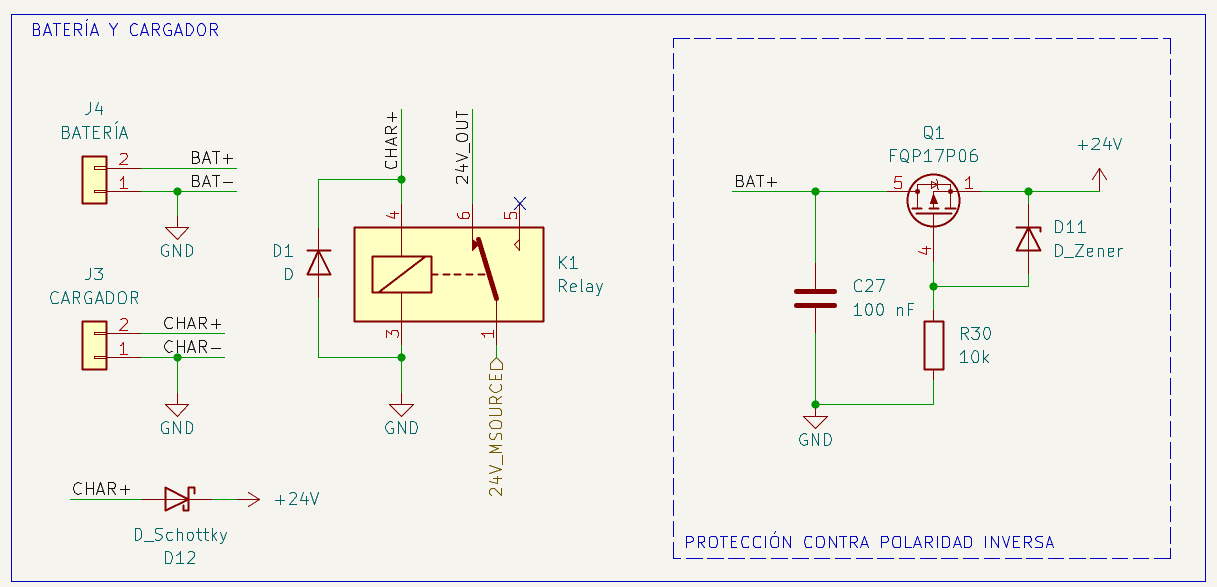
\includegraphics[width=\linewidth]{Recursos/Imagenes/ImagenesDisenoElectronico/EntradaProteccion.png}
	\end{minipage}\hfill
	\begin{minipage}{0.5\textwidth}
		\centering
		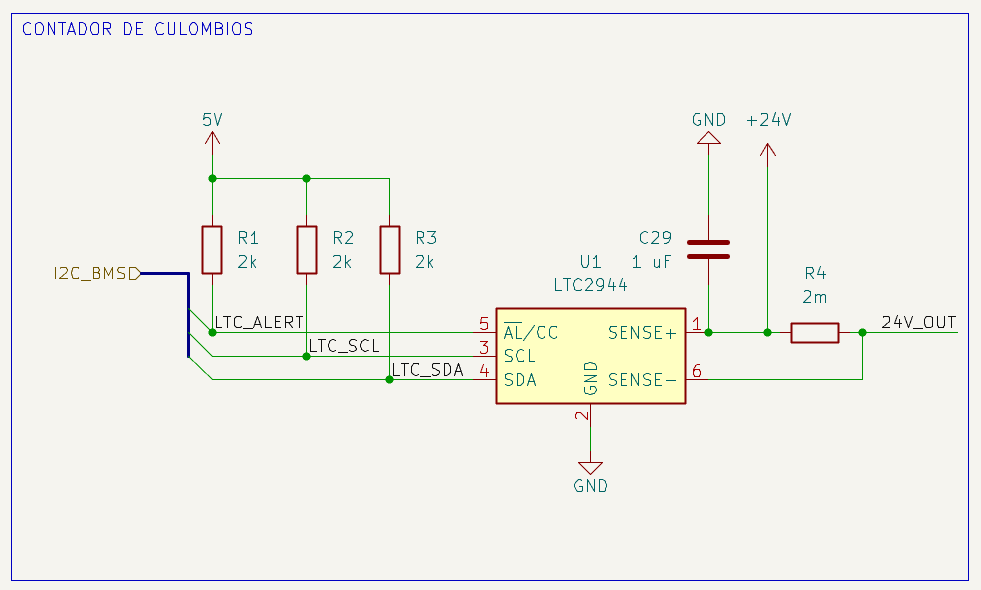
\includegraphics[width=\linewidth]{Recursos/Imagenes/ImagenesDisenoElectronico/ContadorCulombios.png}
	\end{minipage}
	\par\medskip
	
	\raggedright
	\footnotesize \textit{Nota.} Elaboración propia.
	\label{fig:EntradaProteccion}
\end{figure}

\subsection{Supresión de sobretensiones y filtrado pasivo contra interferencias}

La línea de alimentación destinada a los circuitos sensibles de control y adquisición de datos se protege mediante un integrado LTC4364, que actúa como supresor de picos de voltaje y limitador de corriente. Este circuito controla dos transistores MOSFET de canal N conectados en serie: el primero funciona como un diodo ideal que bloquea el retorno de corriente desde los condensadores internos hacia la batería, mientras que el segundo regula el paso de energía para amortiguar sobrevoltajes y limitar la corriente máxima en la entrada.
Los límites de protección se ajustan con divisores de voltaje formados por resistencias de precisión. El corte por bajo voltaje se fija con resistencias de $260\text{ k}\Omega$, $9\text{ k}\Omega$ y $10\text{ k}\Omega$, interrumpiendo el paso de energía si el voltaje de entrada cae por debajo de $18.35\text{ V}$ para evitar la descarga profunda de las baterías. Por otro lado, la protección por sobrevoltaje desconecta la carga si la entrada supera los $34.88\text{ V}$, protegiendo el sistema contra picos de tensión o fallas en cargadores industriales. En caso de transitorios prolongados, el voltaje de salida se limita a $33.75\text{ V}$ mediante un divisor con resistencias de $130\text{ k}\Omega$ y $5\text{ k}\Omega$ conectado al pin de retroalimentación. Si ocurre un cortocircuito o una sobrecorriente continua, el integrado mide la caída de voltaje en una resistencia de $5\text{ m}\Omega$, limita la corriente a $10\text{ A}$ y activa un temporizador por condensador para desconectar la salida y proteger el cableado.
A la salida del limitador, se coloca un filtro pasa bajas pasivo en tipo $\pi$. Este consta de una bobina toroidal de $4.7\text{ }\mu\text{H}$ (con corriente de saturación mayor a $12\text{ A}$) junto a dos condensadores electrolíticos de baja ESR de $470\text{ }\mu\text{F}$ a $50\text{ V}$, colocados en paralelo con condensadores cerámicos para altas frecuencias. Este filtro elimina el ruido electromagnético y entrega un voltaje estable en la línea de $24\text{ V}$ para las siguientes etapas de regulación.

%%%--------------------------------------------------------------------------------------------%%%
%%%--------------------------------------------------------------------------------------------%%%

\begin{figure}[H]
	% Fuerza la alineación izquierda y quita los ":" después del número
	\captionsetup{justification=raggedright, singlelinecheck=false, labelsep=none}
	
	\caption[.]{} 
	
	\textit{.} \par\medskip
	
	\centering
	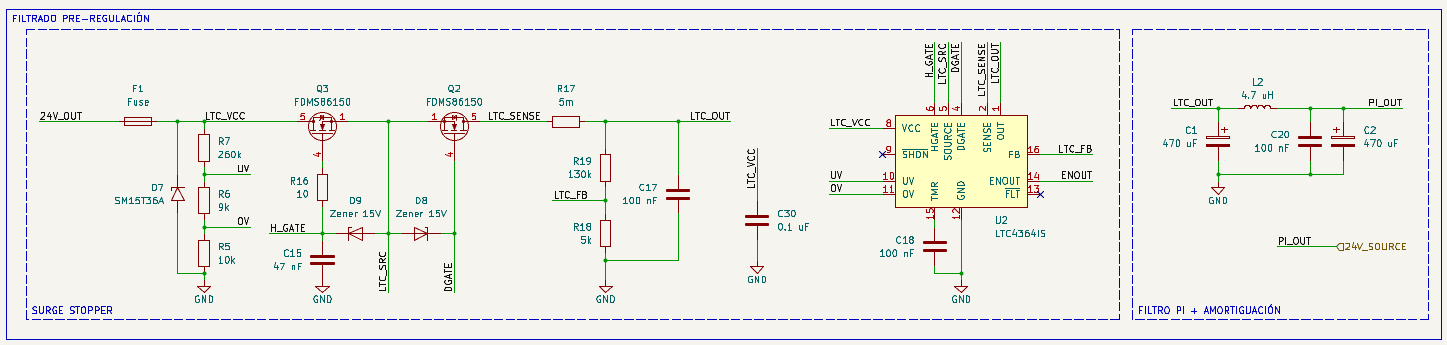
\includegraphics[width=\textwidth]{Recursos/Imagenes/ImagenesDisenoElectronico/FiltroPI.png} \par\medskip
	
	\raggedright
	\footnotesize \textit{Nota.} Elaboración propia.
	\label{fig:FiltroPI}
\end{figure}

%%
%%%--------------------------------------------------------------------------------------------%%%
%%%--------------------------------------------------------------------------------------------%%%

\subsection{Conversión reductora intermedia y distribución de rieles lógicos limpios}

Para alcanzar una elevada eficiencia energética global y evitar la sobrecarga térmica que resultaría de una reducción lineal directa desde $24\text{ V}$ hasta voltajes lógicos de $5.0\text{ V}$ y $3.3\text{ V}$, el sistema emplea una arquitectura híbrida de conversión distribuida en dos fases. En la primera fase, un convertidor conmutado síncrono, modelo TPS54540, se encarga de reducir el voltaje de la barra limpia de $24\text{ V}$ a un nivel intermedio de $6.80\text{ V}$, con capacidad para entregar hasta $5\text{ A}$ de manera continua. 
El ajuste de la frecuencia de oscilación de este regulador se establece en aproximadamente $500\text{ kHz}$ mediante una resistencia de $200\text{ k}\Omega$ conectada al pin de sincronismo, mientras que la tensión intermedia se fija mediante una red de retroalimentación formada por resistencias de $15\text{ k}\Omega$ y $2\text{ k}\Omega$ con una referencia interna de $0.80\text{ V}$, de acuerdo con la expresión:
\begin{equation}
V_{\text{intermedio}} = 0.80 \cdot \left(1 + \frac{15.0\text{ k}\Omega}{2.0\text{ k}\Omega}\right) = 6.80\text{ V}
\end{equation}   
El inductor principal para esta etapa reductora se calcula considerando una corriente de salida de $5\text{ A}$ y un factor de rizado de corriente de $0.30$, seleccionándose un componente blindado de $6.8\text{ }\mu\text{H}$ con una corriente de saturación de $8.5\text{ A}$. 
En la segunda fase, la barra intermedia de $6.80\text{ V}$ alimenta las entradas de dos reguladores lineales de baja caída de potencial (LDO) de la familia LM1084. El primer dispositivo, en su variante fija de $5.0\text{ V}$, absorbe una caída de tensión de apenas $1.80\text{ V}$ para generar la línea de $5.0\text{ V}$ destinada a la computadora monoplaca, las etapas digitales del microcontrolador y los sensores principales. La baja caída de voltaje reduce la potencia disipada por efecto Joule en el encapsulado a valores manejables mediante el plano de cobre de la placa de circuito. A continuación, el segundo regulador lineal, en su variante de $3.3\text{ V}$, se alimenta directamente desde la barra limpia de $5.0\text{ V}$ con una caída de $1.70\text{ V}$ para suplir los circuitos lógicos de baja tensión. Ambos reguladores incorporan diodos Schottky en antiparalelo conectados entre sus terminales de salida y entrada, asegurando una vía de descarga para los condensadores de desacoplo durante el apagado del robot y evitando polarizaciones inversas destructivas en las uniones internas.

%%%--------------------------------------------------------------------------------------------%%%
%%%--------------------------------------------------------------------------------------------%%%

\begin{figure}[H]
	% Fuerza la alineación izquierda y quita los ":" después del número
	\captionsetup{justification=raggedright, singlelinecheck=false, labelsep=none}
	
	\caption[.]{}
	
	\textit{.}\par\medskip
	
	\centering
	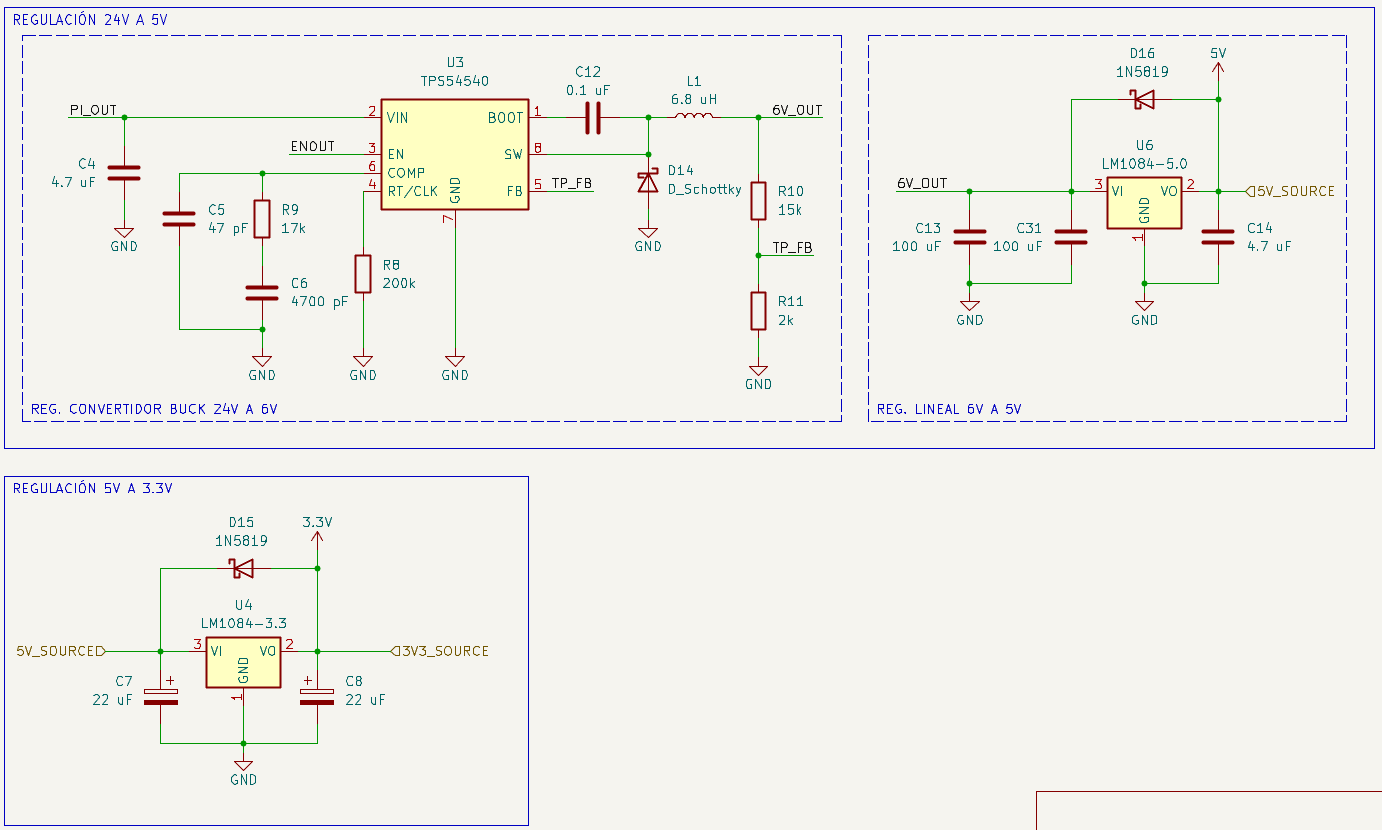
\includegraphics[width=\textwidth]{Recursos/Imagenes/ImagenesDisenoElectronico/2x5V_3_3V.png} \par\medskip
	
	\raggedright
	\footnotesize \textit{Nota.} Elaboración propia.
	\label{fig:2x5V_3_3V}
\end{figure}

%%%
%%%--------------------------------------------------------------------------------------------%%%
%%%--------------------------------------------------------------------------------------------%%%

\subsection{Etapa conmutada de potencia dedicada para servomotores de dirección}

Los servomotores digitales encargados del viraje de las ruedas delanteras demandan corrientes transitorias elevadas que pueden alcanzar valores combinados de hasta $4.6\text{ A}$ durante maniobras sobre terreno irregular o grava. La conexión de estas cargas inductivas sobre la misma línea de alimentación de los circuitos de procesamiento provocaría fluctuaciones de voltaje capaces de reiniciar la computadora de control. Por este motivo, se implementa una etapa de potencia independiente conectada directamente a la barra de actuadores de $24\text{ V}$, constituida por un segundo convertidor conmutado TPS54540.

Este regulador secundario se ajusta a una frecuencia de conmutación de $500\text{ kHz}$ mediante una resistencia de $200\text{ k}\Omega$, sincronizando su operación con la etapa conmutada principal para evitar frecuencias de batido en el espectro electromagnético. La red resistiva de retroalimentación, integrada por resistencias de $13\text{ k}\Omega$ y $2\text{ k}\Omega$, fija una tensión continua de salida de $6.0\text{ V}$ con capacidad para entregar $5\text{ A}$ permanentes, suministrando el torque de retención máximo especificado para los mecanismos de dirección. Para absorber las fuertes demandas de corriente al arrancar los motores internos de los servos, la salida dispone de un banco capacitivo local formado por dos condensadores electrolíticos de $470\text{ }\mu\text{F}$ en paralelo con condensadores cerámicos de $100\text{ nF}$, logrando una reserva energética inmediata de $940\text{ }\mu\text{F}$.

%%%--------------------------------------------------------------------------------------------%%%
%%%--------------------------------------------------------------------------------------------%%%

\begin{figure}[H]
	% Fuerza la alineación izquierda y quita los ":" después del número
	\captionsetup{justification=raggedright, singlelinecheck=false, labelsep=none}
	
	\caption[.]{}
	
	\textit{.}\par\medskip
	
	\centering
	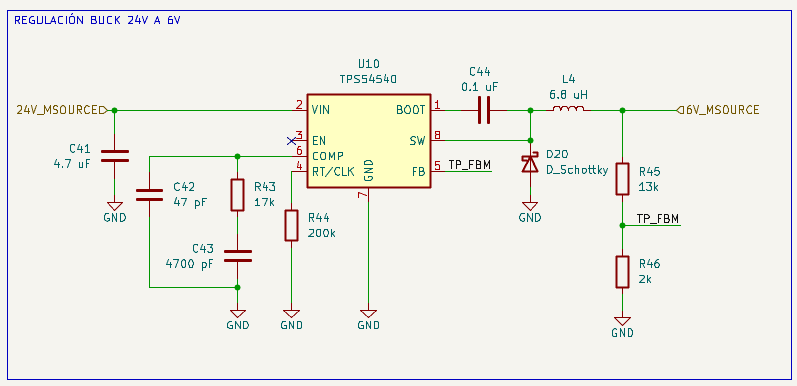
\includegraphics[width=\textwidth]{Recursos/Imagenes/ImagenesDisenoElectronico/BuckServo.png} \par\medskip
	
	\raggedright
	\footnotesize \textit{Nota.} Elaboración propia.
	\label{fig:BuckServo}
\end{figure}

%%%
%%%--------------------------------------------------------------------------------------------%%%
%%%--------------------------------------------------------------------------------------------%%%


\subsection{Fuente variable de instrumentación meteorológica con lazo de seguimiento activo}

La instrumentación exterior montada en la estación móvil abarca transductores con diferentes requerimientos de alimentación, los cuales pueden operar con niveles de $3.3\text{ V}$, $5.0\text{ V}$ o $12.0\text{ V}$. Para energizar estos instrumentos con el menor nivel de ruido electromagnético posible y sin generar una excesiva disipación térmica en el regulador lineal final, se implementa una topología de seguimiento activo con control por lazo híbrido.

El circuito emplea un convertidor reductor conmutado síncrono modelo LMR33630 como etapa de prerregulación, cuya salida alimenta a un regulador lineal ajustable de bajo ruido modelo LM1085. Un transistor bipolar PNP (2N3906) mide continuamente la diferencia de potencial entre la entrada y la salida del circuito LM1085, inyectando corriente correctiva en el nodo de retroalimentación del integrado conmutado. Este mecanismo de control dinámico hace que el convertidor prerregulador ajuste automáticamente su voltaje de salida a un nivel que supera en exactamente $1.85\text{ V}$ al voltaje de salida regulado hacia los sensores. De este modo, independientemente del voltaje configurado por el operador, el regulador lineal opera siempre por encima de su voltaje de caída mínimo requerido de $1.5\text{ V}$ sin generar disipación innecesaria de calor en el encapsulado.

La selección del nivel de voltaje para la instrumentación exterior se realiza mediante un conmutador rotativo unipolar de tres posiciones que altera la resistencia inferior conectada al terminal de ajuste del regulador LM1085. El voltaje de $3.3\text{ V}$ se obtiene seleccionando una resistencia de $200\text{ }\Omega$, el nivel de $5.0\text{ V}$ con $360\text{ }\Omega$ y el nivel de $12.0\text{ V}$ mediante la combinación en serie de una resistencia de $1\text{ k}\Omega$ y $30\text{ }\Omega$. Como medida de versatilidad operativa, se dispone además de un interruptor de dos polos y dos posiciones que permite conmutar la barra de alimentación meteorológica entre la salida lineal regulada y una conexión directa sin regulación a la barra de $24\text{ V}$, permitiendo el uso de sensores industriales con convertidor interno integrado.

%%%--------------------------------------------------------------------------------------------%%%
%%%--------------------------------------------------------------------------------------------%%%

\begin{figure}[H]
	% Fuerza la alineación izquierda y quita los ":" después del número
	\captionsetup{justification=raggedright, singlelinecheck=false, labelsep=none}
	
	\caption[.]{}
	
	\textit{.}\par\medskip
	
	\centering
	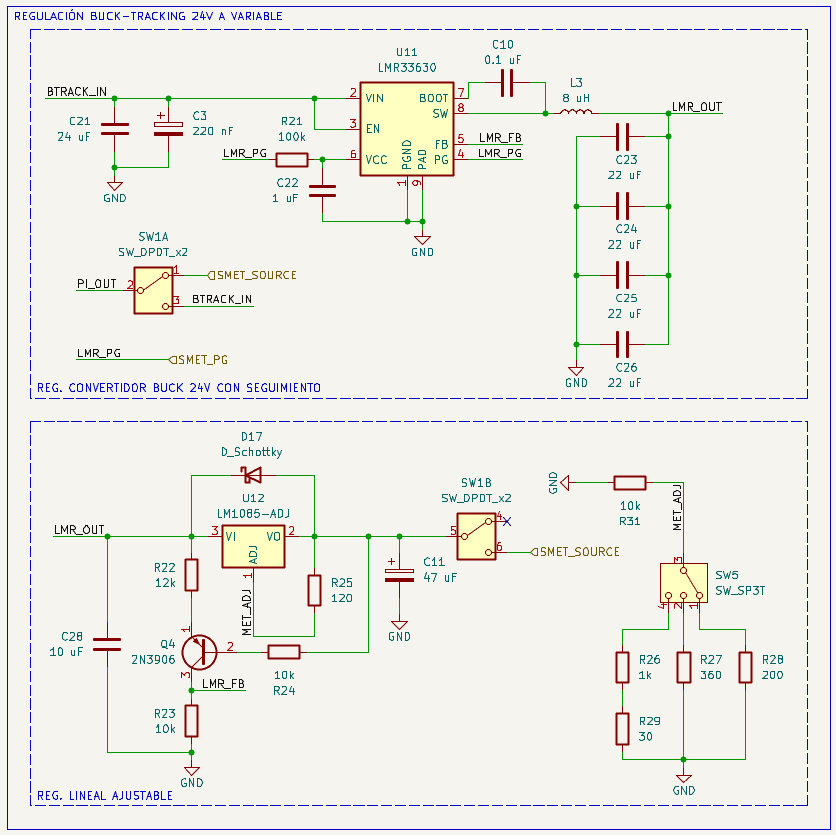
\includegraphics[width=\textwidth]{Recursos/Imagenes/ImagenesDisenoElectronico/BuckTracking.png} \par\medskip
	
	\raggedright
	\footnotesize \textit{Nota.} Elaboración propia.
	\label{fig:BuckTracking}
\end{figure}

%%%
%%%--------------------------------------------------------------------------------------------%%%
%%%--------------------------------------------------------------------------------------------%%%

\subsection{Consumo energético consolidado y dimensionamiento de la batería de alimentación}

Para determinar la capacidad de almacenamiento requerida en la batería del vehículo, se evalúa el balance integral de potencia considerando la totalidad de las cargas eléctricas en su régimen de operación activa simultánea durante las misiones de patrullaje e inspección en campo. Las demandas se desagregan según los diferentes dominios de tensión y funcionamiento del sistema:

En el dominio de procesamiento y control, la computadora monoplaca ejecutando el sistema operativo, los algoritmos de navegación y los servicios de adquisición demanda una potencia media de $5.50\text{ W}$ sobre la línea regulada de $5.0\text{ V}$, mientras que el microcontrolador en tiempo real con sus periféricos lógicos activados consume $1.00\text{ W}$, totalizando $6.50\text{ W}$ en este nivel.

En las etapas de sensores internos y comunicaciones, el arreglo inercial integrado por la unidad primaria de orientación y los dos sensores secundarios demanda $0.35\text{ W}$, el transductor óptico rotativo junto a su red de polarización requiere $0.50\text{ W}$, el receptor satelital de posicionamiento consume $0.35\text{ W}$ y el transceptor de radiofrecuencia de largo alcance promedia un consumo de $2.00\text{ W}$ al considerar un régimen continuo de recepción con ráfagas periódicas de transmisión a un vatio de potencia radiada sobre la banda de $915\text{ MHz}$, sumando un total de $3.20\text{ W}$ sobre las líneas de $5.0\text{ V}$ y $3.3\text{ V}$.

En el dominio de instrumentación meteorológica externa, el piranómetro de precisión clase A acoplado al canal solar, el anemómetro de velocidad y dirección del viento y la sonda termo-higrométrica exterior demandan conjuntamente una potencia permanente de $4.80\text{ W}$ a través de la fuente de seguimiento activo.

En el dominio de potencia motriz, el régimen dinámico típico sobre terreno firme con pendiente moderada implica que el motorreductor de tracción M5, operando bajo consigna de avance continuo a torque nominal, demanda una potencia sostenida de $48.0\text{ W}$ en la barra de $24\text{ V}$. Por su parte, los motores paso a paso de elevación y orientación, alternando fases de ajuste angular fino con fases de retención estática pasiva a corriente reducida, junto a los dos servomotores frontales ejecutando correcciones intermitentes de dirección sobre la barra conmutada de $6.0\text{ V}$, absorben una potencia media combinada de $13.2\text{ W}$.

Considerando un factor de rendimiento medio del $90\%$ en las cadenas de conversión conmutada que abastecen a las cargas lógicas y los sensores de baja tensión, la potencia media total requerida en los bornes de la batería alcanza:

\begin{equation}
P_{\text{total}} = 48.0\text{ W} + 13.2\text{ W} + \frac{6.50\text{ W} + 3.20\text{ W} + 4.80\text{ W}}{0.90} \approx 77.3\text{ W}
\end{equation}

A una tensión nominal de descarga de $24.0\text{ V}$, la corriente media continua entregada por la batería se calcula como:

\begin{equation}
I_{\text{media}} = \frac{P_{\text{total}}}{V_{\text{nominal}}} = \frac{77.3\text{ W}}{24.0\text{ V}} \approx 3.22\text{ A}
\end{equation}

El requerimiento de diseño del proyecto exige garantizar una autonomía operativa ininterrumpida de al menos $1\text{ h}$ sin necesidad de recarga externa en campo. Para preservar la vida útil de las celdas y evitar su envejecimiento acelerado, se define una profundidad de descarga máxima admisible del $80\%$, un rendimiento de eficiencia coulómbica de $0.95$ y un factor de seguridad técnica de $1.25$ para tolerar incrementos transitorios de fricción mecánica en el terreno o caídas de rendimiento por temperatura ambiental. La capacidad nominal requerida para la batería se determina mediante la expresión:

\begin{equation}
C_{\text{bat}} = \frac{I_{\text{media}} \cdot t_{\text{autonomía}}}{\text{DoD} \cdot \eta_{\text{batería}}} \cdot S_f = \frac{3.22\text{ A} \cdot 1.0\text{ h}}{0.80 \cdot 0.95} \cdot 1.25 \approx 5.30\text{ A}\cdot\text{h}
\end{equation}

En términos de acumulación energética equivalente, la capacidad calculada representa:

\begin{equation}
E_{\text{bat}} = C_{\text{bat}} \cdot V_{\text{nominal}} = 5.30\text{ A}\cdot\text{h} \cdot 24.0\text{ V} \approx 127.2\text{ W}\cdot\text{h}
\end{equation}

A partir de estos valores y considerando la disponibilidad comercial en configuraciones en serie de elementos de iones de litio con $6$ celdas (6S), se establece una capacidad de placa estandarizada de $6.0\text{ Ah}$, equivalente a $144\text{ Wh}$ de energía disponible. Este dimensionamiento asegura un margen de autonomía real cercano a $70\text{ min}$ en condiciones de operación continua, absorbiendo con holgura los picos de corriente transitoria de hasta $11.55\text{ A}$ que ocurren durante el arranque simultáneo de los actuadores, sin comprometer la estabilidad térmica ni activar la protección por bajo voltaje del sistema.


\end{document}